\documentclass[a4paper,11pt,titlepage]{jsarticle}


\usepackage{docmute}
\usepackage{braket}%ブラケット関係のやつ
\usepackage[dvipdfmx]{graphicx}%画像関係のやつ
\usepackage[dvipdfmx]{color}
\usepackage{here}%よくわからん
\usepackage{bm}%ベクトル関係のやつ
\usepackage{amsmath} %数学関係のやつ
\usepackage{listings} %プログラムソースのinclude
\usepackage{color}
% \usepackage{scalefnt}
 
\lstset{ 
  basicstyle={\ttfamily},
  identifierstyle={\small},
  commentstyle={\smallitshape},
  keywordstyle={\small\bfseries},
  ndkeywordstyle={\small},
  stringstyle={\small\ttfamily},
  frame={tb},
  breaklines=true, 
  columns=[l]{fullflexible},
  numbers=left,
  xrightmargin=0zw,
  xleftmargin=3zw,
  numberstyle={\scriptsize},
  stepnumber=1,
  numbersep=1zw,
  lineskip=-0.5ex
} %listingsの設定

\numberwithin{equation}{section} %上手い式の数振り
\setcounter{tocdepth}{3} %subsubsectionまで目次に表示



\begin{document}

  \section{レーザーと物質との相互作用を支配する物理}
  
  % \subsection{レーザー強度}
  % レーザーの強度を示すパラメーターとして規格化強度と呼ばれるパラメータが存在し、
  % これは電子の最大揺動速度と光速の比として定義される。
  % \begin{equation}
  %   a_0 = \frac{v_{\rm max}}{c}
  % \end{equation}
  % ここで$v_{\rm max}$は電子の最大揺動速度、$c$は光速を表す。
  % レーザー電磁場が直線変更であるとして、レーザー電場の
  \subsection{相対論的な電子の運動}
  CGS単位系を用いて電子の相対論的な運動方程式を記述すると
  \begin{equation}
    \label{eq:1}
    \frac{d\textit{\textbf{p}}}{dt} = e(\textit{\textbf{E}} + \frac{1}{c} 
    \textit{\textbf{v}} \times \textit{\textbf{B}})
  \end{equation}
  と表される。ここで、$\textit{\textbf{p}} = \gamma_e m_e \textit{\textbf{v}}$
  は電子の運動量を表し、$\textit{\textbf{v}}$は電子の速度を表す。
  また、$\gamma_e = \{ 1-(\frac{v}{c})^2 \}^{-\frac{1}{2}}$はローレンツ因子である。
  \textit{\textbf{E}}、\textit{\textbf{B}}はレーザー電場及び、磁場を表している。
  +y方向へレーザーが伝播すると仮定し、ベクトルポテンシャルを
  $\textit{\textbf{A}} = (\delta a_0 \textrm{cos}\phi,
   0、(1-\delta^2)^{\frac{1}{2}}a_0 \textrm{sin}\phi)$
  で表す。(\ref{eq:1})より、$(p_x、p_y、p_z)$と$(x、y、z)$は以下のように表される。
  \begin{equation}
  \label{eq:2}
    \left\{
      \begin{array}{ll}
        p_x = \delta a_0 \textrm{cos}\phi & \\
        p_y = \frac{a_0^2}{4}[1 + (2\delta^2 - 1)\textrm{cos2}\phi ] & \\
        p_z = (1-\delta^2)^{\frac{1}{2}}
      \end{array}
    \right.
  \end{equation}
  
  \begin{equation}
    \label{eq:3}
      \left\{
        \begin{array}{ll}
          x = \delta a_0 \textrm{sin}\phi & \\
          y = \frac{a_0^2}{4}[\phi + (\delta^2 - \frac{1}{2})\textrm{sin2}\phi ] & \\
          z = -(1-\delta^2)^{\frac{1}{2}} a_0 \textrm{cos}\phi 
        \end{array}
      \right.
    \end{equation}
  \begin{figure}[H]
    \begin{center}
      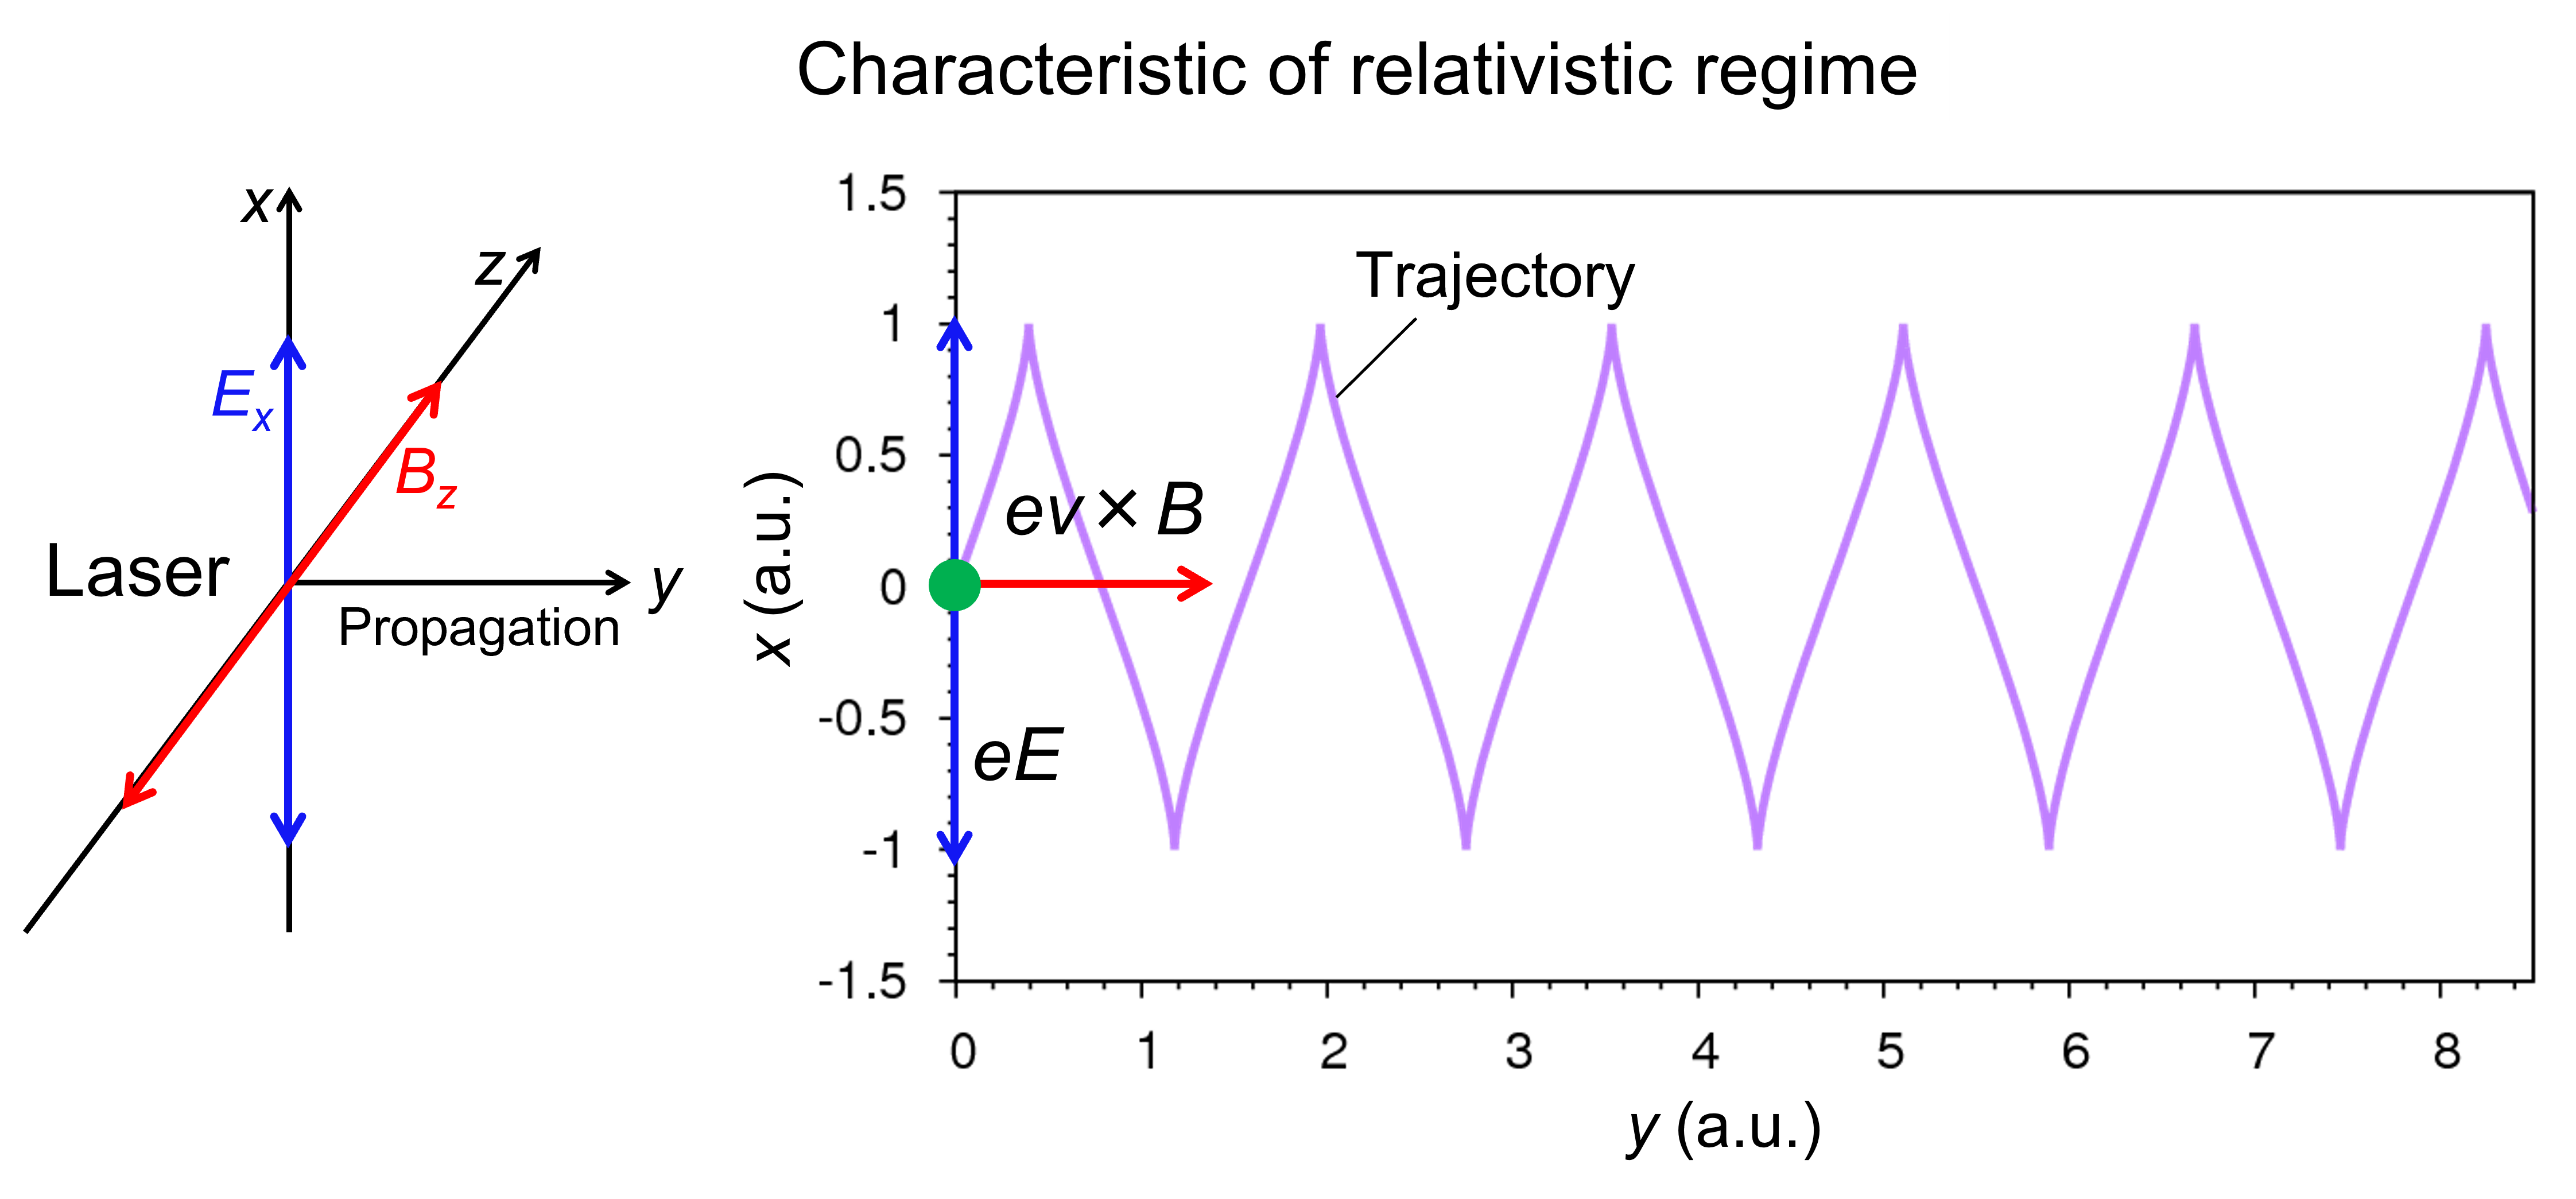
\includegraphics[keepaspectratio,width=\linewidth]{./image/2-1/2-1_propagation.png}
      \label{}
      \caption{
        直線偏光のレーザーが照射された場合の電子軌道を(x、y)平面に描かせた図。レーザーは+y方向に伝播する。
        電子は+y方向にローレンツ力の磁場成分を受けて動く。また、レーザー電場によってx方向に振動を行う。
        (Study of nonlinear structures and dynamics in collisionless plasmas created by the 
        interaction between high power laser and cluster medium より引用)
      }
    \end{center}
  \end{figure}   
  (\ref{eq:3})から分かる通り、規格化強度$a_0$が1より大きい相対論領域において、電子の運動はy方向が支配的となる。
  \subsection{分散関係及びカットオフ密度}
  \rm Maxwell方程式は電場を$\bm{E}$、磁場を$\bm{B}$、電流密度を$\bm{j}$として
  \begin{eqnarray}
    \label{eq:4}
    \nabla \times \textit{\textbf{E}} &=& 
    -\frac{1}{c}\frac{\partial \textbf{\textit{\textbf{B}}}}{\partial t}\\
    \label{eq:5}
    \nabla \times \textit{\textbf{B}} &=& \frac{4\pi}{c} 
    \textbf{\textit{j}} +\frac{1}{c}\frac{\partial \textit{\textbf{B}} }{\partial t}
  \end{eqnarray}
  で与えられる。ここでcは光速を表し、y方向に伝播する電磁波を考えると
  \begin{eqnarray}
    \label{eq:6}
    \textit{\textbf{E}}&=&E_0 e^{i(ky-\omega_L t) \textit{\textbf{x}}}\\
    \label{eq:7}
    \textit{\textbf{B}}&=&B_0 e^{i(ky-\omega_L t) \textit{\textbf{z}}}
  \end{eqnarray}
  で与えられる。ここで$\omega_L$は電磁場(レーザー)の周波数、\textit{k}は波数である。
  これらを(\ref{eq:4})、(\ref{eq:5})のMaxwell方程式に代入すると
  \begin{eqnarray}
    \label{eq:8}
    ckE&=&\omega_L B\\
    \label{eq:9}
    ikB&=&\frac{4\pi}{c}j + \frac{i\omega_L}{c} \textit{E}
  \end{eqnarray}
  (\ref{eq:8})、(\ref{eq:9})より\textit{B}を消去すると以下の式
  \begin{equation}
    \label{eq:10}
    j=\frac{i(c^2 k^2 -\omega_L^2)}{4\pi \omega_L}E
  \end{equation}
  が得られる。ここで\textit{i}は虚数単位を表す。
  また、一方で電子の運動方程式については、(\ref{eq:1})より、電子の初速を0とすると
  \begin{equation}
    \label{eq:11}
    m_e \frac{\textit{dv}}{\textit{dt}}=-e\textit{E}
  \end{equation}
  となり、この式より
  \begin{equation}
    \label{eq:12}
    \textit{v}=-{\frac{e^2 n_e}{m_e} \frac{E}{i\omega_L}}
  \end{equation}
  となる。ここで電子密度を$n_e$とすると、電流密度$j$は$j=en_e v$で表され、
  (\ref{eq:12})より
  \begin{equation}
    \label{eq:13}
    j=-\frac{e^2 n_e}{m_e} \frac{E}{i\omega_L}
  \end{equation}
  となる。(\ref{eq:10})と(\ref{eq:13})を比較することで
  \begin{equation}
    \label{eq:14}
    \omega_L^2={\omega_p}^2+c^2 k^2
  \end{equation}
  が得られ、これがプラズマ中における電磁場の分散関係となる。ここで$\omega_p$は
  プラズマ周波数と呼ばれ、
  \begin{equation}
    \label{eq:15}
    \omega_p = \sqrt{\frac{4\pi n_e e^2}{m_e}}
  \end{equation}
  で表される。また、式(\ref{eq:14})を$k$について解くことで
  \begin{equation}
    \label{eq:16}
    k=\frac{1}{c} \sqrt{\omega_L^2 - {\omega_p}^2}
  \end{equation}
  これより、$\omega_p > \omega_L$の場合、プラズマ内部での電磁波の波数$k$が虚数となり、電磁波が指数関数的に減衰することが分かる。
  この臨界密度のことを特にカットオフ密度と呼び、一般に$n_c$で表記する。
  \begin{equation}
    \label{eq:17}
    n_c=\frac{m_e \omega_L^2}{4\pi e^2}
  \end{equation}
  またこの時の電場\textit{E}は
  \begin{equation}
    \label{eq:18}
    E\propto \rm{exp}(\frac{i}{c} \sqrt{\omega_L^2 - {\omega_p}^2})z
  \end{equation}
  で表されるため、レーザー電場の大きさが1/\textit{e}になる長さ$\delta$は
  \begin{equation}
    \label{eq:19}
    \delta = \frac{c}{\sqrt{{\omega_p}^2-{\omega_L}^2}}
  \end{equation}  
  となる。特に${\omega_p}^2>>{\omega_L}^2$のような高密度プラズマでは
  \begin{equation}
    \label{eq:20}
    \delta = \frac{c}{\omega_p}
  \end{equation}
  となる。この$\delta$をスキン長(表皮距離)と呼ぶ。
  また、相対論領域の高密度プラズマを扱う場合、ローレンツ因子がかかる。
  \begin{equation}
    \label{eq:21}
    \omega_p=\sqrt{\frac{4\pi ne^2}{m\gamma}}
  \end{equation} 
  


  \subsection{レーザーの輻射圧}
  光波には輻射圧があり、特にプラズマ中に加えられるとき、これをポンデロモーティブ力と呼ぶ。
  ポンデロモーティブ力はレーザーとプラズマとの相互作用における一次の力であり、
  非線形現象を説明する重要な物理機構である。この導出は、粒子が従う運動方程式(\ref{eq:11})における一次のオーダーを考えればよい。
  非線形領域における1個の粒子に作用する力の時間平均\textit{f}は次式で表される。
  \begin{equation}
    \label{eq:22}
    f = - \frac{1}{4} \frac{e^2}{m_e \omega_L^2} \nabla E^2
  \end{equation}
  $E^2 = 2 \braket{ \textbf{E}^2 }$ ($\braket{}$は時間平均)を用いると、
  \begin{equation}
    \label{eq:23}
    f = - \frac{\omega_p^2}{\omega_L^2} \nabla \frac{\braket{\textbf{E}^2}}{8\pi}
  \end{equation}
  この力はイオン、電子と電荷に関係なく同じ方向に働く。

  \subsection{クラスターとの相互作用}%クーロン爆発とか両極性膨張とか自己相似解とか
  高強度レーザーをサブミクロンのクラスター(分子が分子間力によって凝集したもの\cite{m3})に照射した場合に
  クラスターの電子は剥ぎ取られ、クラスターは正の電荷を帯び、静電気力によって膨張する。
  このクラスターのクーロン爆発は(A)熱的な膨張(B)両者の中間(C)ピュアなクーロン爆発の3種類に分類される。\cite{Kishi}
  \begin{figure}[H]
    \begin{center}
      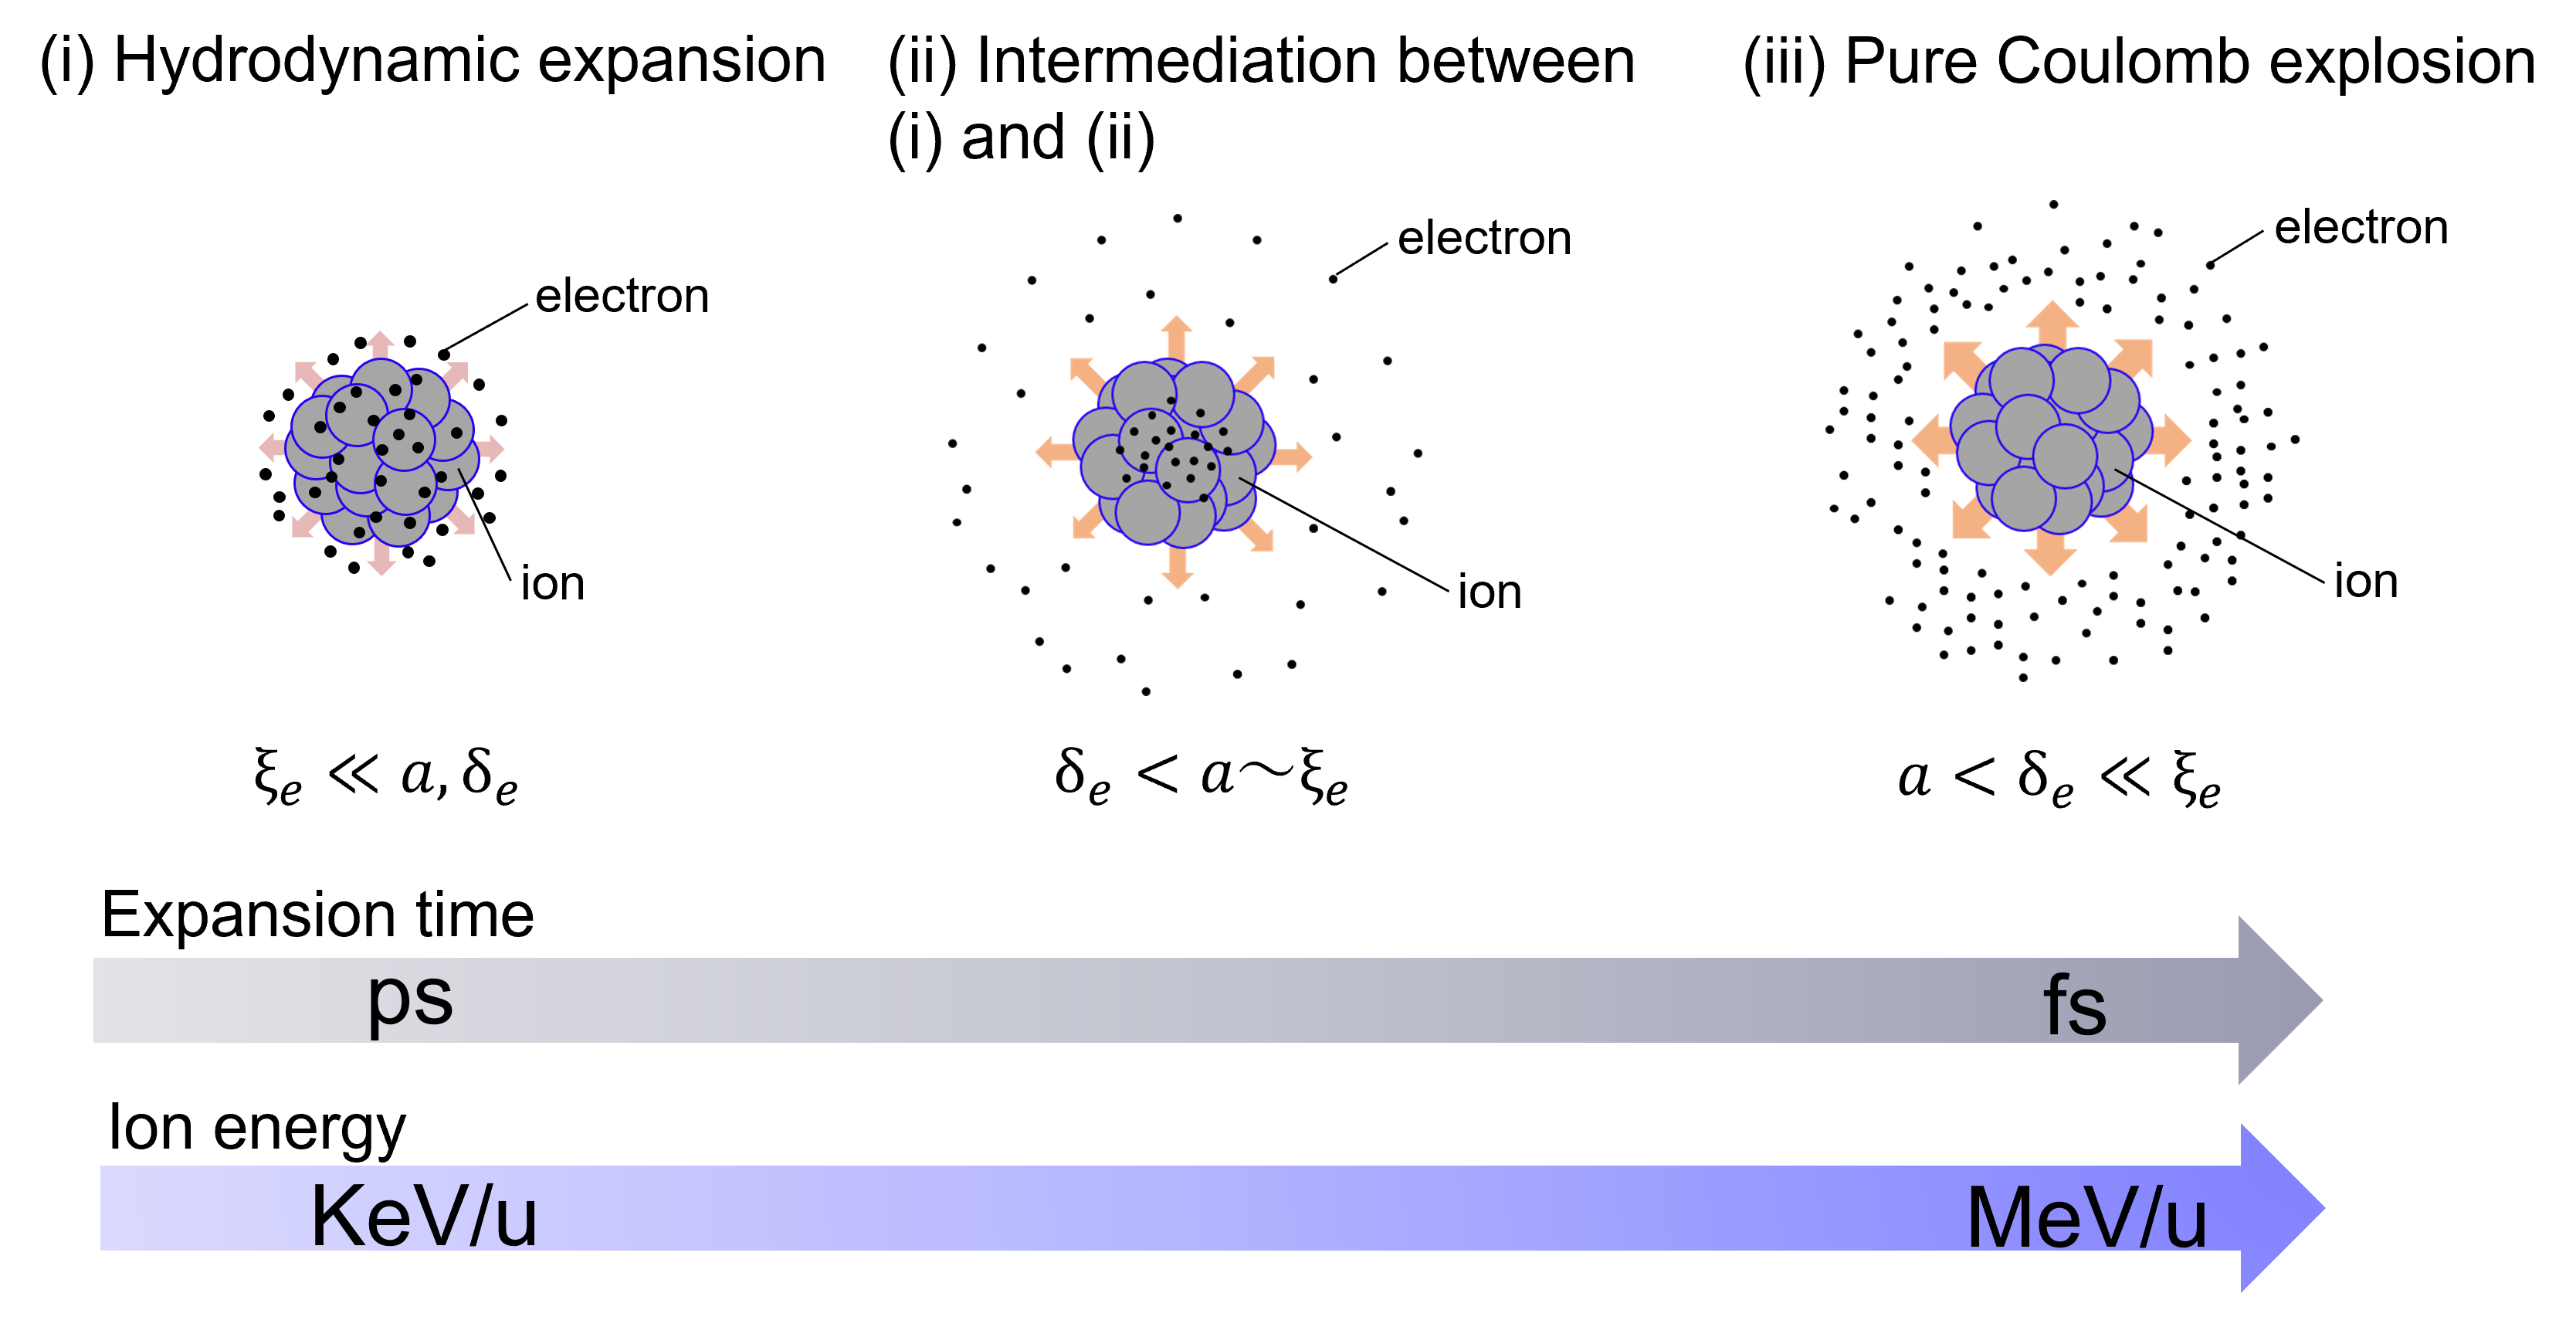
\includegraphics[keepaspectratio,width=\linewidth]{./image/2-1/2-1_explosion.png}
      \caption{
        クラスターにおけるクーロン爆発の分類
      }
      \label{fig:2-4}
    \end{center}
  \end{figure} 
  ここでは、$a$をクラスター半径、$\delta = e/\omega_p$をスキン長、$\xi_e$を周回長とする。\\
    \bf{(A) 熱的な膨張:$\xi_e << a,\delta_e$}\\
   \rm{周回長$\xi_e$がクラスター半径a、および、
  スキン長$\delta_e$よりもはるかに小さい場合は、
  レーザー電場により振動された電子がクラスター表面の周囲に存在する。この時、
  図\ref{fig:2-4}(A)に示すように
  クラスター表面付近の電子は音速で流体力学的に膨張する。}\\
  \\
  \bf{(B) 両者の中間:$\delta_e < a\sim \xi_e$}\\
   \rm{次に、スキン長 $\delta_e$ がクラスター半径 a より小さく、
  周回長$\xi_e$がクラスター半径 a に近い場合
  は、レーザー場はクラスターの周辺領域とのみ相互作用する。この時、
  図 \ref{fig:2-4}(B) に示すようにクラスターの周辺領域は
  クーロン爆発を受け、クラスターの中心は流体力学的に膨張する。}\\
  \\
  \bf{(C) ピュアなクーロン爆発:$a<\delta_e <\xi_e$}\\
   \rm{最後に、周回長 $\xi_e$ がクラスター半径a、および、スキン長$\delta_e$よりも
  はるかに大きい場合は、 図\ref{fig:2-4}(C)に示すように、クラスターのすべての電子は
  クラスターから完全に剥がされて、クラスター
  イオンの反発力によりピュアなクーロン爆発を受ける。}\\
  \subsection{平行極板間における電磁波の伝搬}
  ロッドターゲット間を伝播する電磁波を考察するための基礎理論として、
  2枚の平行な完全導体極板間の領域における波動の伝搬を考察する。波動の伝搬領域を図\ref{fig:2-5_導波管}に示す。
  \begin{figure}[H]
    \begin{center}
      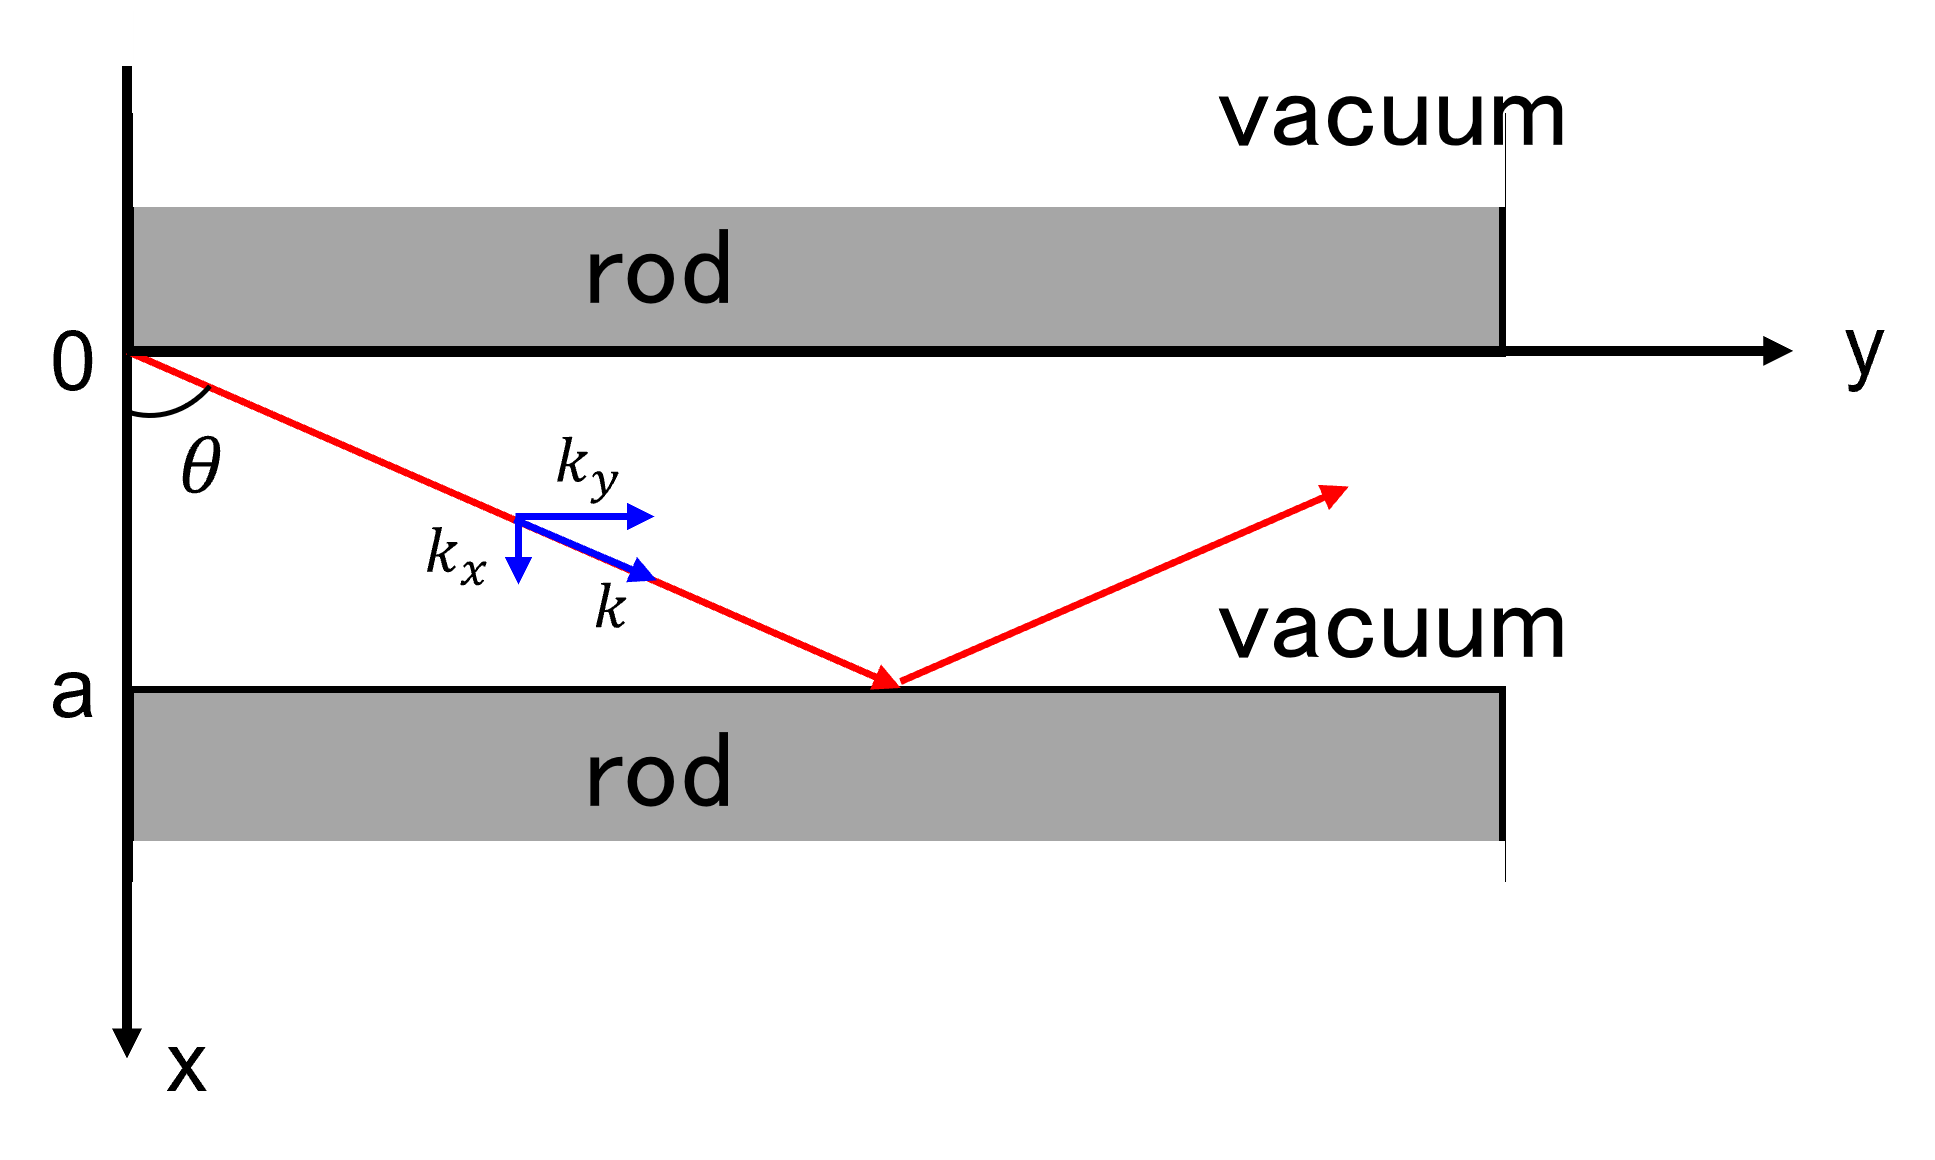
\includegraphics[scale=0.6]{./image/2-5/2-5_導波管.png}
      \caption{
        \label{fig:2-5_導波管}
        2枚の平行極板間の波動伝搬。$k$は入射した波動の波数である。
      }
    \end{center}
  \end{figure} 
  $x$軸と角$\theta$をなす$xy$平面内の波動は、$x=a$にある極板表面に到達した後、
  完全反射し$x$軸と$-\theta$の角をなして伝搬する。したがって、伝搬を表す指数因子は
  \begin{eqnarray}
    \label{eq:2-5-1}
    & e^{i[k(x \cos \theta + y \sin \theta ) - \omega_L t ] }  \nonumber \\
    & e^{i[k( - x \cos \theta + y \sin \theta ) - \omega_L t ] }
  \end{eqnarray}
  となる。ここで$k$は$k=2\pi/\lambda_0$($\lambda_0$:電磁波の波長)を満たす波数、$\omega_L$は角周波数である。このような波動には2つの偏波の可能性が考えられる。1つは電場$E$が$z$軸に平行な場合で、
  TE波(transverse electric wave)と呼ばれ、もう1つは磁場が$z$軸に平行な場合でTM(transverse magnetic wave)波と呼ばれる。
  以降に行うシミュレーションとの兼ね合いから、今回伝播する偏波はTM波であると仮定し、導出を行う。
  すなわち磁場は
  \begin{equation}
    \label{eq:2-5-2}
    \bm{B} = \bm{e_z} \left( B_1 e^{i[k(x \cos \theta + y \sin \theta ) - \omega_L t ] }
                  + B_2 e^{i[k(-x \cos \theta + y \sin \theta ) - \omega_L t ] }    \right)    
  \end{equation}
  と表す。ここで、磁場の境界条件より導体極板に平行な磁場$B_z$は境界面で0になることから、
  $x=0$で$B_z=0$となり、
  \begin{equation}
    \label{eq:2-5-3}
    B_1 = - B_2
  \end{equation}
  同様に$x=a$で$B_z=0$となるので、
  \begin{equation}
    \label{eq:2-5-4}
            B_1 e^{i[k(a \cos \theta + y \sin \theta ) - \omega_L t ] }
          - B_1 e^{i[k(-a \cos \theta + y \sin \theta ) - \omega_L t ] }    
          = 0 
  \end{equation}
  これを整理して
  \begin{equation}
    \label{eq:2-5-5}
     \left(  e^{ ika \cos \theta } - e^{ -ika \cos \theta } \right) e^{ i \left( ky \sin \theta - \omega_L t  \right) } 
          = 0 
  \end{equation}
  すなわち
  \begin{equation}
    \label{eq:2-5-6}
     ka \cos \theta = n \pi 
  \end{equation} 
  を満たす。したがって式(\ref{eq:2-5-2})は式(\ref{eq:2-5-6})を用いて
  \begin{eqnarray}
    \label{eq:2-5-7}
    B_x &=& 0  \\
    \label{eq:2-5-8}
    B_y &=& 0 \\
    \label{eq:2-5-9}
    B_z &=&  2 B_1 \cos ( \frac{n \pi}{a} x ) e^{ i \left( k_y y - \omega_L t  \right) }
  \end{eqnarray}
  ここで、$ \bm{\nabla} \times \bm{B} = - \frac{1}{c^2} \frac{\partial \bm{E} }{ \partial t } $ より、
  \begin{eqnarray}
    \label{eq:2-5-10}
    E_x &=& 2 B_1 \frac{c^2}{\omega_L} k_y \cos( \frac{n\pi}{a} x ) e^{ i \left( k_y y  - \omega_L t  \right) }  \\
    \label{eq:2-5-11}
    E_y &=& -2 i B_1  \frac{c^2}{\omega_L} \frac{n\pi}{a} \sin ( \frac{n \pi}{a} x ) e^{ i \left( k_y y - \omega_L t  \right) } \\
    \label{eq:2-5-12}
    E_z &=& 0
  \end{eqnarray}
  ただし、ここでは、波数の各方向の成分を$k_x = k \cos \theta $、$k_y = k \sin \theta $とする。
  式(\ref{eq:2-5-7})から(\ref{eq:2-5-12})は実空間において
  \begin{eqnarray}
    \label{eq:2-5-13}
    B_x &=& 0  \\
    \label{eq:2-5-14}
    B_y &=& 0 \\
    \label{eq:2-5-15}
    B_z &=&  2 B_1 \cos ( \frac{n \pi}{a} x ) \cos \left( k_y y - \omega_L t  \right) \\
    \label{eq:2-5-16}
    E_x &=& 2 B_1 \frac{c^2}{\omega_L} k_y \cos( \frac{n\pi}{a} x ) \cos \left( k_y y - \omega_L t  \right) \\
    \label{eq:2-5-17}
    E_y &=& -2 B_1  \frac{c^2}{\omega_L} \frac{n\pi}{a} \sin ( \frac{n \pi}{a} x ) \sin \left( k_y y - \omega_L t  \right) \\
    \label{eq:2-5-18}
    E_z &=& 0
  \end{eqnarray}
  と書き直すことができる。
  このとき、分散関係は
  \begin{equation}
    \label{eq:2-5-19}
    k^2 = k_x^2 + k_y^2
  \end{equation}
  であり、この条件の下で、式(\ref{eq:2-5-6})を満たす$\theta$を探すことで、伝搬可能な電磁波の波数(入射角度)が分かる。
  例えば、$n=1$のとき式(\ref{eq:2-5-6})は$\cos \theta = \lambda_0 / 2 a $となるが、$\lambda_0$が増すにつれて、
  分散関係を満たすために$k_y^2$は負でなければならない。
  このとき、(\ref{eq:2-5-7})~(\ref{eq:2-5-12})より、波は指数関数的に減衰してしまう。
  言い換えれば、$n = 1$における伝搬可能な最大の波長は$2a$であると言える。
  \newpage 
\end{document}

